\begin{enumerate}
\item $AB$ is tangent to the circles $CAMN$ and $NMBD$. $M$ lies between $C$ and $D$ on the line $CD$, and $CD$ is parallel to $AB$. The chords $NA$ and $CM$ meet at $P$; the chords $NB$ and $MD$ meet at $Q$. The rays $CA$ and $DB$ meet at $E$. Prove that $PE = QE$.\hfill(IMO 2000)
    \item Let $ABCD$ be a convex quadrilateral with perpendicular diagonals. If $AB = 20$, $BC = 70$, and $CD = 90$, then what is the value of $DA$?\hfill(PRERMO 2014)
    \item In a triangle with integer side lengths, one side is three times as long as a second side, and the length of the third side is $17$. What is the greatest possible perimeter of the triangle?\hfill(PRERMO 2014)
    \item In a triangle $ABC$, $X$ and $Y$ are points on the segments $AB$ and $AC$, respectively, such that $ AX : XB = 1 : 2 $ and $ AY : YC = 2 : 1.$If the area of triangle $AXY$ is $10$, then what is the area of triangle $ABC$?\hfill(PRERMO 2014)
    \item Let $XOY$ be a triangle with $\angle XOY = 90\degree$. Let $M$ and $N$ be the midpoints of legs $OX$ and $OY$, respectively. Suppose that $XN = 19$ and $YM = 22$. What is $XY$?\hfill(PRERMO 2014)
\item $PS$ is a line segment of length 4 and $O$ is the midpoint of $PS$. A semicircular arc is drawn with $PS$ as diameter. Let $X$ be the midpoint of this arc. $Q$ and $R$ are points on the arc $PXS$ such that $QR$ is parallel to $PS$ and the semicircular arc drawn with $QR$ as diameter is tangent to $PS$. What is the area of the region $QXROQ$ bounded by the two semicircular arcs?\hfill(PRERMO 2012)
\item $O$ and $I$ are the circumcentre and incentre of $\triangle ABC$ respectively. Suppose $O$ lies in the interior of $\triangle ABC$ and $I$ lies on the circle passing through $B$, $O$, and $C$. What is the magnitude of $\angle BAC$ in degrees?\hfill(PRERMO 2012)
\item In $\triangle ABC$, we have $AC = BC = 7$ and $AB = 2$. Suppose that $D$ is a point on line $AB$ such that $B$ lies between $A$ and $D$ and $CD = 8$. What is the length of the segment $BD$?\hfill(PRERMO 2012)
\item In rectangle $ABCD$, $AB = 5$ and $BC = 3$. Points $F$ and $G$ are on line segment $CD$ so that $DF = 1$ and $GC = 2$. Lines $AF$ and $BG$ intersect at $E$. What is the area of $\triangle ABE$?\hfill(PRERMO 2012)
\item A triangle with perimeter 7 has integer side lengths. What is the maximum possible area of such a triangle?\hfill(PRERMO 2012)
\item $ABCD$ is a square and $AB$ = 1 Equilateral triangles $AYB$ and $CXD$ are drawn such that $X$ and $Y$ are inside the square.What is the length of $XY$?\hfill(PRERMO 2012)
\item The figure below shows a broken piece of a circular plate made of glass.
    
	  
		\begin{figure}[h!]
    \centering
	    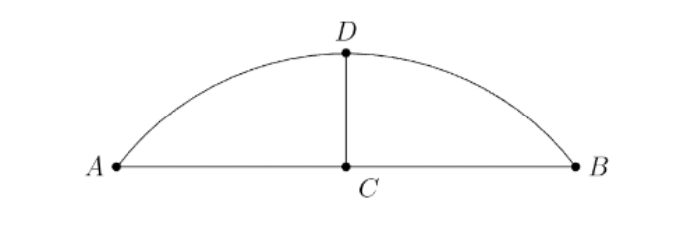
\includegraphics[width=\columnwidth]{olympiad/figs/permo.jpg}
    \end{figure}



    $ C $ is the midpoint of $ AB $, and $ D $ is the midpoint of arc $ AB $. Given that $ AB = 24 $ cm and $ CD = 6 $ cm, what is the radius of the plate in centimeters? (The figure is not drawn to scale.)\hfill(PRERMO 2015)

    \item A $ 2 \times 3 $ rectangle and a $ 3 \times 4 $ rectangle are contained within a square without overlapping at any interior point, and the sides of the square are parallel to the sides of the two given rectangles. What is the smallest possible area of the square? \hfill(PRERMO 2015)

    \item What is the greatest possible perimeter of a right-angled triangle with integer side lengths if one of the sides has length 12? \hfill(PRERMO 2015)

    \item In rectangle $ ABCD $, $ AB = 8 $ and $ BC = 20 $. Let $ P $ be a point on $ AD $ such that $ \angle BPC = 90\degree $. If $ r_1, r_2, r_3 $ are the radii of the incircles of triangles $ APB, BPC $, and $ CPD $, what is the value of $ r_1 + r_2 + r_3 $? \hfill(PRERMO 2015)


\item In the acute-angled triangle $ABC$, let $D$ be the foot of the altitude from $A$, and $E$ be the midpoint of $BC$. Let $F$ be the midpoint of $AC$. Suppose $ \angle BAE = 40\degree $. If $ \angle DAE = \angle DFE $, what is the magnitude of $ \angle ADF $ in degrees?\hfill(PRERMO 2015)

\item The circle $ \omega $ touches the circle $ \Omega $ internally at $ P $. The center $ O $ of $ \Omega $ is outside $ \omega $. Let $XY$ be a diameter of $ \Omega $ which is also tangent to $ \omega $. Assume $ PY > PX $. Let $ PY $ intersect $ \omega $ at $ Z $. If $ YZ = 2PZ $, what is the magnitude of $ \angle LPYX $ in degrees? \hfill(PRERMO 2015)
	\item On each side of an equilateral triangle with side length $n$ units, where $n$ is an integer,$1 \leq n \leq 100$ , consider $n - 1$ points that divide the side into $n$ equal segments.Through these points, draw lines parallel to the sides of the triangle, obtaining a net of equilateral triangles of side length one unit. On each of the vertices of these small triangles, place a coin head up. Two coins are said to be adjacent if the distance between them is $1$ unit. A move consists of flipping over any three mutually adjacent coins. Find the number of values of $n$ for which it is possible to turn all coins tail up after a finite number of moves.\hfill(IOQM 2015)


	\item In an equilateral triangle of side length $6$, pegs are placed at the vertices and also evenly along each side at a distance of $1$ from each other. Four distinct pegs are chosen from the $15$ interior pegs on the sides (that is, the chosen ones are not vertices of the triangle) and each peg is joined to the respective opposite vertex by a line segment.If $N$ denotes the number of ways we can choose the pegs such that the drawn linesegments divide the interior of the triangle into exactly nine regions, find the sum ofthe squares of the digits of $N$.\hfill(IOQM 2015)		
	\item In a triangle $ABC$, let $E$ be the midpoint of $AC$ and $F$ be the midpoint of $AB$. The medians $BE$ and $CF$ intersect at $G$. Let $Y$ and $Z$ be the midpoints of $BE$ and $CF$, respectively. If the area of triangle $ABC$ is 480, find the area of triangle $GYZ$.\hfill(IOQM 2015)
	    \item The six sides of a convex hexagon $A_{1}A_{2}A_{3}A_{4}A_{5}A_{6}$ are colored red. Each of the diagonals of the hexagon is colored either red or blue. If $N$ is the number of colorings such that every triangle $A_{i}A_{j}A_{k}$ , where $1 \leq i < j < k \leq 6$ , has at least one redside, find the sum of the squares of the digits of $N$ .\hfill(IOQM 2015)
    \item Let $X$ be the set of all even positive integers $n$ such that the measure of the angle of some regular polygon is $n$ degrees. Find the number of elements in $X$ .\hfill(IOQM 2015)
    
    \item Let $ABCD$ be a unit square. Suppose $M$ and $N$ are points on $BC$ and $CD$, respectively, such that the perimeter of triangle $MCN$ is $2$. Let $O$ be the circumcenter of triangle $MAN$, and $P$ be the circumcenter of triangle $MON$. If $\left(\frac{OP}{OA}\right)^2 = \frac{m}{n}$ for some relatively prime positive integers $m$ and $n$, find the value of $m + n$.\hfill(IOQM 2015)
    
    \item Let $ABC$ be a triangle in the $xy$-plane, where $B$ is at the origin $\brak{0, 0}$. Let $BC$ be produced to $D$ such that $BC : CD = 1 : 1$, $CA$ be produced to $E$ such that $CA : AE = 1 : 2$, and $AB$ be produced to $F$ such that $AB : BF = 1 : 3$. Let $G\brak{32, 24}$ be the centroid of triangle $ABC$ and $K$ be the centroid of triangle $DEF$. Find the length $GK$.\hfill(IOQM 2015)
    
    \item In the coordinate plane, a point is called a lattice point if both of its coordinates are integers. Let $A$ be the point $\brak{12, 84}$. Find the number of right-angled triangles $ABC$ in the coordinate plane where $B$ and $C$ are lattice points, having a right angle at the vertex $A$ and whose incenter is at the origin $\brak{0, 0}$.\hfill(IOQM 2015)
    
    \item A trapezium in the plane is a quadrilateral in which a pair of opposite sides are parallel. A trapezium is said to be non-degenerate if it has positive area. Find the number of mutually non-congruent, non-degenerate trapeziums whose sides are four distinct integers from the set $\cbrak{5, 6, 7, 8, 9, 10}$.\hfill(IOQM 2015)
    
    \item In triangle  $ABC$, point $ A_1 $ lies on side $ BC $ and point $B_1$ lies on side $ AC $. Let  $P$ and $ Q $ be points on segments 
$AA_1$ and $BB_1 $, respectively, such that   $PQ \parallel AB$.

Let
 $P_1$ be a point on line  $PB_1$ such that $B_1$ lies strictly between 
$P$ and $P_1$, and $\angle PP_1C$ = $\angle BAC$. Similarly, let $Q_1$ 
be a point on line $QA_1$ such that $A_1$ lies strictly between $Q$ and 
$Q_1$, and $ \angle CQ_1Q$ = $\angle CBA $.
Prove that points $P, Q, P_1,$ and $Q_1$ are concyclic.
\hfill(IMO 2019)


\item
 Let $I$ be the in center of acute triangle $ABC$ with $AB$ $\neq AC$. 
The incircle $\omega$ of $ABC$ is tangent to sides $ BC$, $CA$, and $AB$
 at points $D$,  $E$, and $F$, respectively. 


The line 
through $D$ perpendicular to $EF$ meets $\omega$ again at $R$. Line $AR$
 meets $omega$ again at $P$. The circumcircles of triangles $PCE$ and 
$PBF$ meet again at $Q$.

Prove that lines $DI$ and $PQ$ meet on the line through $ A$ that is perpendicular to $AI$.
\hfill(IMO 2019)
\item consider the convex quadrilateral ABCD.The point P is the interior of ABCD.The following ratio equalities hold:
\begin{align}
\angle PAD: \angle PBA: \angle DPA =1:2:3 = \angle CBP: \angle BAP: \angle BPC.
\end{align} 
prove
 that the following three lines meet in a point:the internal bisectors 
of angles $\angle ADP$ and $\angle PCB$ and the perpendicular bisector 
of segment AB
\hfill(IMO 2020)
\item Prove that there exists a positive constant c such that the following statement is true:
Consider an integer n\textgreater1, and a set S of n points in the plane such that the distance between
any
 two different points in S is at least 1. It follows that there is a 
line l separating S such that the distance from any point of S to l is 
at least $cn^\frac{-1}{3}$
(A line l separates a set of points S if some segment joining two points in S crosses l.)
Note. Weaker results with  replaced by $cn^\alpha$ may be awarded points depending on the value of the constant $ \alpha$ \textgreater1/3.
   \hfill(IMO 2020)
\item Let D be an interior point of the acute triangle ABC with AB \textgreater AC so that $\angle DAB = \angle CAD$.The point E on the segment AC satisfies $\angle ADE=\angle BCD$,the point F on the segment AB satisfies $\angle FDA=\angle DBC$,and the point X on the line AC satisfies CX=BX. let $O_{1}$ and $O_{2}$ be the circumcentres of the triangles ADC and EXD,respectively.Prove that the lines BC,EF,and $O_{1} O_{2}$ are concurrent
 \hfill(IMO 2021)
\item Let r be a circle with centre I,and ABCD a convex quadrilateral such that each of the segments AB,BC,CD and DA is a tangent to r.Let \ohm be the circumcircle of the triangle AIC.The extension of BA beyond A meets \ohm at X,and the extension of BC beyond C meets \ohm at Z.The extensions of AD and CD beyond D meet \ohm at Y and T,respectively.Prove that
\begin{align}
    AD+DT+TX+XA=CD+DY+YZ+ZC
\end{align}
 \hfill(IMO 2021)
 \item
Let $ABCDE$  be a convex pentagon such that  $BC = DE$.  Assume that there is a point  $T$  inside  $ABCDE$ with  $TB = TD$,  $TC = TE$  and  $\angle{ABT} = \angle{TEA}$.  Let line  $AB$  intersect 
lines $CD$  and  $CT$  at points  $P$  and $Q$,  respectively. Assume that the points  $P, B, A, Q$  occur on their line in that order. Let line  $AE$  intersect lines  $CD$  and  $DT$  at points  $R$  and  $S$,  respectively. Assume 
that the points $ R, E, A, S $ occur on their line in that order. Prove that the points $ P, S, Q, R $ lie on a circle. \hfill(IM0 2022)
\item
Let  $ABC$ be an acute-angled triangle with  $AB \leq AC$. Let $\Omega$  be the circumcircle of  $ABC$.  Let  $S$ be the midpoint of the arc  $CB$  of  $\Omega$ containing $A$.  The perpendicular from $A$  to  $BC$ meets  $BS$  at  $D$  and meets  $\Omega$  again at$E \neq A$. The line through $
D$ parallel to  $BC$  meets line  $BE$ at  $L$.  Denote the circumcircle of triangle  $BDL$  by  $\omega$.  Let  $\omega$  meet  $\Omega$  again at  $P \neq B$.Prove that the line tangent to $\omega$ at  $P$  meets line $BS$  on the internal angle bisector of  $\angle{BAC}$. \hfill(IMO 2023)
\item
Let  $ABC$  be an equilateral triangle. Let $A_{1}, B_{1}, C_{1}$  be interior points of  $ABC$  such that $ BA_{1} = A_{1}C, CB_{1} = B_{1}A, AC_{1} = C_{1}B,$  and $\angle{BAC} + \angle{CB_{1}A} + \angle{AC_{1}B} = 480^{\circ}.$  Let $ BC_{1}$ and $CB_{1}$  meet at $A_{2}$,  let  $CA_{1}$ and  $A
C_{1}$  meet at  $B_{2}$,  and let  $AB_{1}$ and  $BA_{1}$  meet at  $C_{2}$. Prove that if triangle  $A_{1}B_{1}C_{1}$  is scalene, then the three circumcircles of triangles $AA_{1}A_{2}, BB_{1}B_{2}$  and  $CC_{1}C_{2}$ all pass through two common points.
$\brak{\text{Note: no 2 sides have equal length.}}$ \hfill(IMO 2023)
\item
Let  $ABC$  be a triangle with $ AB \leq AC \leq BC $.  Let the incentre and incircle of triangle   $ABC$  be  $I$ and  $\omega$, respectively. Let $X$ be the point on line  $BC$  different from  $C$  such that the line   through  $X$  parallel to  $AC$  is tangent to  $\omega$.  Similarly, let  $
Y$ be the point on line  $BC$  different from  $B$  such that the line through  $Y$ parallel to  $AB$  is tangent to  $\omega$.  Let $AI$  intersect the circumcircle of  triangle $ABC$  again at  $P \neq A$. Let  $K$  and $L$  be the midpoints of  $AC$  and  $AB$,  respectively.  Prove that  $\angle{KIL} + \angle{YPX} = 180^{\circ}.$ \hfill(IMO 2024)
\item Three points $ X, Y, Z $ are on a straight line such that $ XY = 10 $ and $ XZ = 3 $. What is the product of all possible values of $ YZ $?\hfill(Prermo 2013)

\item Let $ AD $ and $ BC $ be the parallel sides of a trapezium $ ABCD $. Let $ P $ and $ Q $ be the midpoints of the diagonals $ AC $ and $ BD $. If $ AD = 16 $ and $ BC = 20 $, what is the length of $ PQ $?\hfill(Prermo 2013)

\item In a triangle $ ABC $, let $ H $, $ I $, and $ O $ be the orthocenter, incenter, and circumcenter, respectively. If the points $ B $, $ H $, $ I $, and $ C $ lie on a circle, what is the magnitude of $ \angle BOC $ in degrees?\hfill(Prermo 2013)

\item Let $ ABC $ be an equilateral triangle. Let $ P $ and $ S $ be points on $ AB $ and $ AC $, respectively, and let $ Q $ and $ R $ be points on $ BC $ such that $ PQRS $ is a rectangle. If $ PQ = \sqrt{3} \times PS $ and the area of $ PQRS $ is $ \frac{28}{3} $, what is the length of $ PC $?\hfill(Prermo 2013)

\item Let $ A_1, B_1, C_1, D_1 $ be the midpoints of the sides of a convex quadrilateral $ ABCD $ and let $ A_2, B_2, C_2, D_2 $ be the midpoints of the sides of the quadrilateral $ A_1B_1C_1D_1 $. If $ A_2B_2C_2D_2 $ is a rectangle with sides 4 and 6, then what is the product of the lengths of the diagonals of $ ABCD $?\hfill(Prermo 2013)

\item Let $ S $ be a circle with center $ O $. A chord $ AB $, not a diameter, divides $ S $ into two regions $ R_1 $ and $ R_2 $. Let $ S_1 $ be a circle with center in $ R_1 $ touching $ AB $, the circle $ S $ internally. Let $ S_2 $ be a circle with center in $ R_2 $ touching $ AB $ at $ Y $, the circle $ S $ internally, and passing through the center of $ S $. The point $ X $ lies on the diameter passing through the center of $ S_2 $, and $ \angle YXO = 30^\circ $. If the radius of $ S_2 $ is 100, then what is the radius of $ S $?\hfill(Prermo 2013)

\item In a triangle $ ABC $ with $ \angle BCA = 90^\circ $, the perpendicular bisector of $ AB $ intersects segments $ AB $ and $ AC $ at $ X $ and $ Y $, respectively. If the ratio of the area of quadrilateral $ BXYC $ to the area of triangle $ ABC $ is 13:18 and $ BC = 12 $, then what is the length of $ AC $?\hfill(Prermo 2013)
\item $A$ convex hexagon has the property that for a ny pair of opposite sides the distance between their midpoints is $\frac{\sqrt{3}}{2}$ times the sum of their lengths Show that all the hexagon's angles are equal.\hfill(IMO 2003)
\item $ABCD$ is cyclic. The feet of the perpendicula r from $D$ to the lines $AB$, $BC$, $CA$ are $P, Q,R $ respectivel$y$. Show that the angle bisectors of $ ABC$ and $CDA$ meet on the line $AC$ iff $RP = RQ$.\ hfill(IMO 2003)
\item Let $ABC$ be an acute-angled triangle with circumcentre $0$. Let $P$ on $BC$ be the foot o f the altitude from $A$. \\Suppose that $\textless BC S$ $\leq$ $\angle ABC+30^0$. \\Prove that $\textless CAB+\leq cop \angle 90^o$.\hfill(IMO 2001)
\item In a triangle $ABC$, let $AP$ bisect $\angle B AC$, with $P$ on $BC$, and let $BQ$ bisect $\angle A BC$, with $Q$ on $CA$. It is known that $\angle BAC= 60^0$ and that $AB+BP=AQ+QB$. What are the possible angles of triangle $ABC$?\hfill(IMO 2001)
\item $BC$ is a diameter of a circle center $0$. $A$ is any point on the circle with $\angle AOC \textgreater 60^0$. $EF$ is the chord which is the perpendicular bisector of $AO$. $D$ is the midpoint of the minor arc $AB$. The line through $0$ parallel to $AD$ meets $AC$ at $J$. Show that $J$ is the inc enter of triangle $CEF$.\hfill(IMO 2002)
\item $n\textgreater2$ circlesof radius $1$ are drawn in the plane so that no line meets more th an two of the circles. Their centers are $0_{1}, 0_{ 2}\dots0_{n}$. Show that $\sum_{i\textless}$ $1/0_{i }0_{j}\leq \brak{n-1} \frac{\pi}{4}$.\hfill(IMO 2002)
\item In the plane two different points $O$ and $A$ are given.  For each point $X$ of the plane, other than $O$, denote by $a\brak{X}$  the measure of the angle between $OA$ and $OX$ in radians countrclockwise from $OA\brak {O\leq a\brak{X}<2\pi}$. Let $C\brak{X}$ be the circle  with center $O$ and radius of length $\frac {OX+a\brak{X}}{OX}$. each  point  of the plane is colored by one of a finite number of colors. Proveoint $Y$ for which $a\brak{y}>0$ such that color appears on  the circumference of the circle $C\brak{Y}$.\hfill(IMO 1984)
\item Let $ABCD$ be a convex quadrilateral such tha the line $CD$ is a  tangent to the circle on $AB$ as diameter. Prove that the line $AB$ is a tangent to the  circle on $CD$ as diameter if and only if the lines $BC$ and $AD$ are parallel.\hfill(IMO 1984)
\item Let $d$ be the sum of the lengths of all the diagonals of a plane convex polygon with $n$ vertices $\brak{n>3}$,and let $p$ be its perimeter.Prove that.\begin{align*}                                    In-3<\frac{2d}{p}<\myvec{\frac{n}{2}}\myvec{\frac{n+1}{2}}-2,\end{align*}
		Where $\myvec{x}$ denotes the gratest integer not excee    ding $x$  \hfill(IMO 1984)

	
\item let $A$ be one of the two distinct points of intersection of two unequal coplanar tangents to the circles $C_1$ and $C_2$ with centers $ O_1$ and $O_2$, respectively. One of the common tangents to the circles touches $C_1$ at $P_1$ and $C_2$ at $P_2$, while the other touches $C_1$ at $Q_1$ and $C_2$ at $Q_2$.  Let $M_1$ be the midpoint of $P_1Q_1$,$M_2$ be the midpoint of $P_2Q_2$ prove that $\angle O_1AO_2 =\angle M_1AM_2$.\hfill(IMO1983)

     \item $A$ circle has center on the side $AB$ of the cyclic quadrilateral $ABCD$. The other three sides are tangent to the circle. Prove that $AD+BC = AB$.\hfill(IMO 1985)

\item A circle with center $O$ passes through the vertices $A$ and $C$ of triangle $ABC$ and intersects the segments $AB$ and $BC$ again at distinct points $K$ and $N$ respectively. The circumscribed circle of the triangle $ABC$ and $EBN$ intersect at exactly two distinct points $B$ and $M$. Prove that angle $OMB$ is a right angle.\hfill(IMO 1985)
\item $P$ is a point inside a given triangle $ABC.D, E, F$ are the feet of the perpendiculars from $P$ to the lines $BC, CA, AB$ respectively. Find all $P$ for which \\ $\frac{BC}{PD}+\frac{CA}{PE}+\frac{AB}{PF}$ is least. \hfill(IMO 1981)
\item Three congruent circles have a common point $O$ and lie inside     a given triangle. Each circle touches a pair of sides of the triangle. Prove that the incenter and the circumcenter of the triangle and   the point $O$  are collinear\hfill(IMO 1981)     
\item A non-isosceles triangle $A_1 A_2 A_3$ is given with sides $a_1,a_2,a_3$ ($a_i$ is the sid    e opposite $A_i$). For all $i = 1, 2, 3, M_i$ is the midpoint of side $a_i$ and $T_i$ is the point where     the incircle touches side $a_i$. Denote by $S_i$ the reflection. of $T_i$ in the interior bisector of anngle $A_i$. Prove that the lines $M_1,S_1$,$ M_2S_2$ and $M_3S_3$ are concurrent.\hfill(IMO 1982)
 \item The diagonals $AC$ and $CE$ of the regular hexagon $ABCDEF$ are divided by the inner points $M$ and $N$, respectively, so that \begin{align*} \frac{AM}{AC}=\frac{CN}{CE}=r.
                   \end{align*}
 Determine r if $B,$ $M,$ and $N$ are collinear. \hfill(IMO 1982)
 \item Let $S$ be a square with sides of length $100$, and let $L$ be a path with in $S$ which does not meet itself and which is composed of line segments $A_0A_1, A_1A_2,.... A_{n-1}A_1$ with $A_0 \neq A_n$.     Suppose that for every point $P$ of the boundary of $S$ there is a point of $L$ at a distance from $P$ not greater than $\frac{1}{2}$. Prove that there are two points $X$ and $Y$ in  $\&$ such that the distance between $X$ and $Y$ is not greater than $1$, and the length of that part of $L$ which lies between $X$ and $Y$ is not smaller than $198$.\hfill(IMO 1982)
\item A triangle $A_1A_2A_3$ and a point $P_0 $are given in the plane.We define $A_s
    =A_s-3$ for all $s\geq4$ .We construct a set of points $P_1$, $P_2$,$P_3$\dots,such that $P_{k+1}$ is the image of $P_k$ under a rotation with center $A_{k+1}$ through angle $120^\circ$ clockwise $\brak{for \space k=0,1,2,3\dots}$ .Prove that if $P_{1986}$=$P_0$, then thetriangle $A_1A_2A_3$ is equilateral .\hfill(IMO 1986)

    \item Let $A$, $B$ be adjacent vertices of a regular n-gon $\brak{n\leq5}$ in the plane having center at $O$. A triangle $XYZ$, which is congruent to and initially conincides with $OAB$, moves in the plane in such a way that $Y$ and $Z$ each trace out the whole boundary of the polygon, $X$ remaining inside the polygon. Find the locus of $X$.\hfill(IMO 1986)

    \item In an acute-angled triangle $ABC$ the interior bisector of the angle $A$ intersects $BC$ at $L$ and intersects the circumcircle of $ABC$ again at $N$. From point $L$ perpendiculars are drawn to $AB$ and $AC$, the feet of these perpendiculars being $K$ and $M$respectively. Prove that the quadrilateral $AKNM$ and the triangle $ABC$ have equal areas.\hfill(IMO 1987)

    \item Prove that there is no function $f$ from the set of non-negative integers into itself such that $f\brak{f\brak{n}}=n+1987$ for every $n$.\hfill(IMO 1987)

    \item Consider two coplanar circles of radii $R$ and $r$ $\brak{R > r}$ with the same center. Let $P$ be a fixed point on the smaller circle and $B$ a variable point on the lar ger circle. The line $BP$ meets the larger circle again at $C$. The perpendicular $l$ to $BP $ at $P$ meets the smaller circle again at $A$. (If $l$ is tangent to the circle at $P$ then $A = P$)
                 $\brak{i}$ Find the set of values of $BC^2+CA^2+AB^2$ 
                 $\brak{ii}$ Find the locus of the midpoint of $BC$.\hfill(IMO 1988)

\item $ABC$ is a triangle right-angled at $A$, and $D$ is the foot of the altitude from $A$. The straight line joining the incenters of the triangles $ABD$, $ACD$ intersects the sides $AB$, $AC$ at the points $K$, $L$ respectively. $S$ and $T$ denote the areas of the triangles $ABC$ and $AKL$ respectively. Show that $S\geq 2T$.\hfill(IMO 1988)
\item Problem $5$. A configuration of $4027$ points in the plane is called Colombian if it consists of $2013$ red points and $2014$ blue points, and no three of the points of the configuration are collinear. By drawing some lines, the plane is divided into several regions. An arrangement of lines is good for a Colombian configuration if the following two conditions are satisfied:
 * no line passes through any point of the configuration;
* no region contains points of both colours

Find the least value of $k$ such that for any Colombian configuration of $4027$ points, there is a good arrangement of $k$ lines \hfill(Imo 2013)
\item Problem 6. Let the excircle of triangle $ABC$ opposite the vertex $A$ be tangent to the side $BC$ at the point $A_1$. Define the points $B_1$, on $CA$ and $C_1$, on $AB$ analogously, using the excircles opposite $B$ and $C$. respectively. Suppose that the circumcentre of triangle $A_1B_1C_1$, lies on the circumcircle of triangle $ABC$. Prove that triangle $ABC$ is right-angled. \hfill(Imo 2013)
                        
	The excircle of triangle $ABC$ opposite the vertex $A$ is the circle that is tangent to the line segment $BC$, to the ray $AB$ beyond $B$, and to the ray $AC$ beyond $C$. The excircles opposite $B$ and $C$ are similarly defined. \hfill(Imo 2013)
\item problem7 Let $ABC$ be an acute-angled triangle with orthocentre$ H$, and let $W$ be a point on the side $BC$, lying strictly between $B$ and $C$. The points $M$ and $N$ are the fect of the altitudes from $B$ and $C$, respectively. Denote by $w_1$ the circumcircle of $BWN$, and let $X$ be the point on wy such that $WX$ is a diameter of $w_1$ Analogously, denote by $w_2$ the circumcircle of $CWM$. and let $Y$ be the point on such that $WY$ is a diameter of Prove that $X$, $Y$ and Hare collinear. \hfill(Imo 2013)
	
\item Problem 8. Let $ Q_{>0}$ be the set of positive rational mumbers. Let $f: Q_{>0} \rightarrow R$ be a function satisfying the following three conditions:
	\begin{enumerate}
		\item for all $x,y\epsilon  Q>0$, we have $f\brak{x} f\brak{y} \geq  f\brak{xy}$
		\item for all $x,y\epsilon Q>0$,we have$f\brak{x+y} \geq f\brak{x}+f\brak{y}$
		\item there exists a rational number $a> 1$ such that $f\brak{a}=a$.
			
		prove that $F\brak{x}=x$ for all $x \epsilon Q>0$.
	\end{enumerate} \hfill(Imo 2013)			
\item Problem 9. let $n\geq 2$ be an integer. Consider an $n\times n$ chessboard consisting of $n^2$ unit squares. A configuration of $n$ rooks on this board is peaceful if every row and every column contains exactly one rook. Find the greatest positive integer $k$ such that, for each peaceful configuration of $n$ rooks, there is a $k\times k$ square which does not contain a rook on any of its $k^2$ unit squares. \hfill(Imo 2014)
	
\item Problem 10. Convex quadrilateral $ABCD$ has $\angle ABC= \angle CDA = 90 \degree$ Point His the foot of the perpendicular from A to BD. Points S and T lie on sides $AB and AD$, respectively, such that $H$ lies inside triangle $SCT$ and $\angle CHS- \angle CSB = 90 \degree , \angle THC- \angle DTC = 90\degree$ .
	Prove that line $BD$ is tangent to the circumcircle of triangle $TSH$. \hfill(Imo 2014)
\item Problem 4. Points $P and Q$lie on side $BC$ of acute-angled triangle $ABC$ so that $\angle PAB= \angle BCA$ and $\angle CAQ=\angle ABC.$ Points $M$ and $N$ lie on lines $AP$ and $AQ,$ respectively, such that $P$ is the midpoint of $AM,$ and $Q$ is the midpoint of $AN.$ Prove that lines $BM and CN$ intersect on circumcircle of triangle $ABC$ \hfill(Imo 2014)
\item Problem 11. A set of lines in the plane is in general position if no two are parallel and no three pass through the same point. A set of lines in general position cats the plane into regions, some of which have finite area; we call these its finite regions. Prove that for all sufficiently large $n$. in any set of a lines in general position it is possible to colour at least $\sqrt n$ of the lines blue in such a way that none of its finite regions has a completely blue boundary.

	Note: Results with $\sqrt n$ replaced by $c \sqrt n$  will be awarded points depending on the value of the constant $c$. \hfill(Imo 2014)
	
\item Problem 12. We say that a finite set $S$ of points in the plane is balanced if, for any two different points $A and B$ in $S$, there is a point Cin Ssuch that $AC=BC$. We say that $S$ is centre-free if for any three different points $A, B$ and $C$ in $S$, there is no point $P$ in $S$ such that $PA=PB=PC$
	\begin{enumerate} 

\item  Show that for all integers $n\geq3$, there exists a balanced set consisting of $n$ points.

\item  Determine all integers $n\geq3$ for which there exists a balanced centre-free set consisting of $n$ points.
	\end{enumerate}	\hfill(Imo 2015)	
	
\item Problem 13. Determine all triples $\brak{a, b, c}$ of positive integers such that each of the numbers
			 $ ab-c, bc-a,ca-b$\\
		is a  power of $2$\\(A power of 2 is an integer of the form $2^n$,Where $n$ is a non-negative integer). \hfill(Imo 2015)
		
\item Problem 14. Let $ABC$ be an acute triangle with $AB\textgreater AC$ Let I be its circumcircle, $H$ its orthocentre, and $F$ the foot of the altitude from $A$. Let $M$ be the midpoint of $BC$. Let $Q$ he the point on $T$ such that $\angle HQA= 90$, and let $K$ be the point on $T$ such that $\angle HKQ=90\degree.$ Assume that the points$ A, B, C, K and Q$ are all different, and lie on $T$ in this order.

	Prove that the circumcircles of triangles $KQH$ and $FKM$ are tangent to each other. \hfill(Imo2015)
\item Problem 15. Triangle $ABC$ has circumcircle $\ohm$ and circumcentre $O$. A circle $T$ with centre. A intersects the segment $BC$ at points $D and E$, such that $B, D, E $and Care all different and lie on line $BC$ in this onter. Let $F and G $be the points of intersection of $T and \ohm$. such that $A. F B. C and G $lie on \ohm in this order. Let $K $ he the second point of intersection of the circumcircle of triangle $BDF$ and the segment $AB$. Let $L$ be the second point of intersection of the circumcircle of triangle $CGE$ and the segment $CA$
	Suppose that the lines $FKand GL$ are different and intersect at the point $X$. Prove that $X$ lies on the line $AO$. \hfill(Imo 2015)
\item Problem 16. Let $R$ be the set of real numbers. Determine all functions $f:R\rightarrow R$ satisfying the equation
	\begin{align}
		f\brak{x+f\brak{x+y}}+f\brak{xy}=x+f\brak{x+y}+yf\brak{x}
	\end{align}
for all real numbers $x$ and $y$ \hfill(Imo2015)

\item problem17 the sequence $a_1,a_2, \ldots$ of an integers satisfies the following conditions;
	\begin{enumerate}
		\item $1\leq a_{j} \leq2015$ for all $j\geq 1;$
		\item $k+a_{k} \neq l+a_{l}$ for all $1\leq k \textless l.$
	\end{enumerate}	
prove that there exist two positive integers $b and N$ such that

$\mydet {\sum_{j=m+1}^{n} \brak {aj-b} }\leq 1007^2$

for all integers $m and n$ satisfying $n > m\geq N$ \hfill(Imo 2015)
\item Prove that the set $\cbrak{1,2,.........,1989}$ can be expressed as the disjoint union of subsets $A_i$\brak{i=1,2,........,117} such that :
\brak{i} Each $A_i$ contains $17$ elements ;
		\brak{ii} The sum of all the elements in each $A_i$ is the same . \hfill(IMO 1989)


\item In an acute-angled triangle $ABC$ the internal bisector of angle $A$ meets the circumcircle of the triangle again at $A_1$. Points $B_1$ and $C_1$ are defined similarly. Let $A_0$ be the point of intersection of the line $AA_1$ with the external bisectors of angles $B$ and $C$. Points $B_0$ and $C_0$ are defined similarly. Prove that: 

\brak{i} The area of the triangle $A_0$ $B_0C_0$ is twice the area of the hexagon $AC_1BA_1CB_1$

\brak{ii} The area of the triangle $A_0B_0C_0$ is at least four times the area of the triangle $ABC$. \hfill(IMO 1989)

\item Let $n$ and $k$ be positive integers and let $S$ be a set of $n$ points in the plane such that

\brak{i} No three points of $S$ are collinear, and 

\brak{ii} For any point $P$ of $S$ there are at least $k$ points of $S$ equidistant from $P$. \hfill(IMO 1989)

		Prove that: \begin{align*}k < \frac{1}{2} + \sqrt{2n}.\end{align*}

	\item Let $ABCD$ be a convex quadrilateral such that the sides ${AB, AD, BC}$ satisfy $AB= AD + BC$. There exists a point. $P$ inside the quadrilateral at a distance $h$ from the line $CD$ such that $AP= h+ AD$ and $BP= h + BC$. Show that:\begin{align*}
	\frac{1}{\sqrt{h}}\geq\frac{1}{\sqrt{AD}}+\frac{1}{\sqrt{BC}}\end{align*}. \hfill(IMO 1989)


   \item Chords $AB$ and $CD$ of a circle imersect at a point $E$ inside the circle. Let $M$ be an interior point of the segment $EB$. The tangen    t line at $E$ to the circle through $D, E$. and $M$ intersects the lines $BC$ and $AC$ at $F$ and $G$. respectively,                                      If \begin{align*}\frac{AM}{AB}=t \end{align*}      
  find \begin{align*} \frac{EG}{EF}\end{align*}  
	  in terms of t .\hfill(IMO 1990)


      \item Let $n_3$ and consider a set $E$ of $2_{n-1}$ distinct points on a circle. Suppose that exactly $k$ of these points are to he colored black. Such a coloring is $"good"$ if there is at least  one pair of black points such that the interior of one of the ares between them contains exactly in points from $E$. Find the smallest value of $k$ so that every such coloring of $k$ points of $E$ is good \hfill(IMO 1990)


     \item Given an initial integer $n_0 > 1$, two players. $A$ a    nd $B$, choose integers $n_1, n_2 , n_3,.......$ alternately accordi    ng to the following rules:
           Knowing $n_{2k}$, $A$ chooses any integer $n_{2k+2}$ such that \begin{align*} n_{2k}\leq n_{2k+1} \leq n^{2}_2{k} \end{align*}
   Knowing $n_{2k+1}$ , $B$ chooses any integer $n_{2k+2}$ such that \begin{align*}
              \frac{n_{2k+1}}{n_{2k+2}}\end{align*}
  is a prime raised to a positive integer power.
	Plaver $A$ wins the game by choosing the number $1990$: player $B$ wins by choosing the number $1$. For which $n_0$ does:
\brak{a}$A$ have a winning strategy?
\brak{b} $B$ have a winning strategy?
\brak{c} Neither player have a winning strategy?\hfill(IMO 1990)

\item Prove that there exists a convex $1990$-gon with the following     two properties
\brak{a} All angles are equal.
\brak{b} The lengths of the 1990 sides are the numbers $1^2, 2^2, 3^    2$,.....,$1990^2$ in some order.\hfill(IMO 1990)

\item Let $ABC$ be a triangle and $P$ an interior point of $ABC$.     Show that at least one of the angles $\angle{PAB}, \angle{PBC}, \angle{PCA}$ is less than or equal to $30\degree$.\hfill(IMO 1991)

\item Equilateral triangles $ABK$, $BCL$, $CDM$, $DAN$ are constructed inside the square $ABCD$. Prove that the midpoints of the four segments $KL$, $LM$, $MN$, $NK$ and the midpoints of the eight segments $AKBK$, $BL$, $CL$, $CM$, $DM$, $DN$, $AN$ are the twelve vertices of a regular dodecagon.\hfill(Imo 1977).
\item $P$ is a given point inside a given sphere.Three mutually perpendic ular rays from Pintersect the sphere at points $U, V$, and $W$; $Q$ denotes the vertex diagonally opposite to $P$ in the parallelepiped determined by $PU, PV$, and $PW$.     Find the locus of $Q$ for all such triads of rays from $P$\hfill(Imo 1978)
\item In triangle $ABC$, $AB = AC$. A circle is t    angent internally to the circumcircle of triangle $ABC$ and also to sides $AB, AC$ at $P. Q$, respectively. Prove that the midpoint of segment $PQ$ is the center of the incircle of triangle $ABC.$\hfill(Imo 1978)

\item A prism with pentagons $A1 A2 A3 A4 A5$ and $B1 B2 B3 B4 B5$, as top and bottom faces is given. Each side of the two pentagons and each of the line- segments $A,B$ for all $i, j = 1,\ldots,5$, is colored either red or green. Every triangle whose vertices are vertices of the prism and whose sides have all been colored has two sides of a different color. Show that all $10$ sides of the top and bottom faces are the same color.\hfill(Imo 1979) 
\item Two circles in a plane intersect. Let $A$ be one of the points of intersection. Starting simultaneously from $A$ two points move with constant speeds, each point travelling along its own circle in the same sense. The two points return to $A$ simultaneously after one revolution. Prove that there is a fixed point $P$ in the plane such that, at any time, the distances from $P$ to the moving points are equal.\hfill(Imo 1979) 
\item Given a plane $\pi$, a point $P$ in this plane and a point $Q$ not in $\pi$, find all points$R$ in $\pi$ such that the ratio $\brak{QP+PA}/Q R$ is a maximum. \hfill(Imo 1979)
\item Let $I$ be the incenter of triangle $ABC$. Let the incircle of $ABC$ touch the sides $BC$,$CA$, and $AB$ at $K$, $L$, and $M$, respectively.The line through $B$ parallel to $MK$ meets the lines $LM$ and $LK$ at $R$ and $S$, respectively. Prove that angle $RIS$ is acute.\hfill(IMO 1998)

\item Determine all finite sets $S$ of at least three points in the plane which satisfy the following condition:\\for any two distinct points $A$ and $B$ in $S$, the perpendicular bisector of the line segment $AB$ is an axis of symmetry for $S$.\hfill( IMO 1999)

\item Two circles ${G_{1}}$ and ${G_{2}}$ are contained inside the circle $G$, and are tangent to $G$ at the distinct points $M$ and $N$, respectively. ${G_{1}}$ passes through the center of ${G_{2}}$. The line passing through the two points of intersection of ${G_{1}}$ and ${G_{2}}$ meets $G$ at $A$ and $B$. The lines $MA$ and $MB$ meet ${G_{1}}$ at $C$ and $D$, respectively. Prove that $CD$ is tangent to ${G_{2}}$.\hfill(IMO 1999)
                      	
\item ${A_{1}} {A_{2}} {A_{3}}$ is an acute-angled triangle. The foot of the altitude from ${A_{i}}$ is ${K_{i}}$ and the incircle touches the side opposite ${A_{i}}$ at ${L_{i}}$. The line ${K_{1}}{K_{2}}$ is reflected in the line ${L_{1}}{L_{2}}$. Similarly, the line ${K_{2}}{K_{3}}$ is reflected in ${L_{2}}{L_{3}}$ and ${K_{3}}{K_{1}}$ is reflected in ${L_{3}}{L_{1}}$. Show that the three new lines form a triangle with vertices on the incircle.\hfill(IMO 2000)
\item In the convex quadrilateral $ABCD$,the diagonals $AC$ and $BD$ are perpendicular and the oppositesides $AB$ and $DC$ are not parallel.Suppose that thepoint $P$, where the perpendicular bisectors of $AB$and $DC$ meet, is inside $ABCD$. Prove that $ABCD$ is a cyclic quadrilateral ifand only if the triangles$ABP$ and $CDP$ have equalareas.\hfill(IMO 1998) 
\item Let $ABC$ be an acute-angled triangle  with $AB$ $\neq$ $AC$.The circle with diameter $BC$ intersects the sides $AB$ and $AC$ at $M$ and $N$ respectively.Denote by $O$ the midpoint of the side $BC$.The bisector of the angles $<$$BAC$ and $<$$MON$ intersects at $R$.Prove that the circumcircles of the triangles $BMR$ and $CNR$ have a common point on the side $BC$ \hfill(IMO 2004)
 \item In a convex quadrilateral ABCD the diagonal BD does not bisect the angles ABC and CDA.The point P lies inside ABCD and satisfies
 \begin{align*}
 \angle{PBC}=\angle{DBA} and \angle{PDC}=\angle{BDA}.
 \end{align*}
Prove that ABCD is a cyclic quadrilateral if and only if AP=CP \hfill(IMO 2004)
	\item Six points are chosen on the sides of an equilateral triangle $ABC$:
     $A_1$,$A_2$ on $BC$,$B_1$,$B_2$ on $CA$ and $C_1$,$C_2$ on $AB$, such that they are the vertices of a convex hexagon $A_1A_2$ $B_1B_2$ $C_1C_2$ with equal side lengths.Prove that the line $A_1B_2$,$B_1C_2$ and $C_1A_2$ are concurrent.\hfill(IMO 2005)
     \item prove that $x,y,z$ be three positve real such that $xyz$ $\geq{1}$.Prove that                                                            \begin{align*}
\frac{x^5-x^2}{x^5+y^2+z^2} + \frac{y^5-y^2}{x^2+y^5+z^2} + \frac{z^5-z^2} {x^2+y^2+z^5} \geq{0}                                                 \end{align*} \hfill(IMO 2005)
\item Let $ABCD$ be a fixed convex quadrilateral with $BC$ = $DA$ and
    $BC$ not parallel with $DA$. Let two variable points $E$ and $F$ lie of the sides $BC$ and $DA$, respectively and satisfy $BEDF$. The lines $AC$and $BD$ meet at $P$,the lines $BD$ and $EF$ meet at $Q$, the lines $EF$ and $AC$ meet at $R$.Prove that the circumcircles of the triangles $PQR$, as $E$ and $F$ vary,have a common point other than $P$.\hfill(IMO 2005)
 \item In a mathematical competition, in which $6$ problems were posed to the participants, every two of these problems were solved by more than $\frac{2}{5}$ of the contestants. Moreover, no contestant solved all the $6$ problems. Show that there are at least $2$ contestants who solved exactly $5$ problems each.\hfill(IMO 2005)
\item Let $P$ be a regular 2006-gon. A diagonal of $P$ is called good if its endpoints divide the boundary of $P$ into two parts, cach composed of an odd mumber of sides of P.The sides of Pare also called good.Suppose $P$ has been dissected into triangles by 2003 diagonals, no two of which have a common point in the interior of $P$. Find the maximum number  of isosceles triangles having two good sides that could appear in such a configuration\hfill(IMO 2006)
\item Assign to each side $b$ of a convex polygon $P$ the maximum area of a triangle that has $b$ as a side and is contained in $P$. Show that the sum of the areas assigned to the sides of $P$ is at least twice the area of $P$.\hfill(IMO 2006)
\item Consider five points $A,B,C,D$ and $E$ such that $ABCD$ is a parallelogram and $BCED$ is a cycle quadrilateral.Let $l$ be a line passing through A. suppose that $l$ intersts the interior of the segment $DC$ at $F$ and intersects line $BC$ at $G$.suppose also that $EF=EG=EC$. Prove that $l$ is the bisector of angle $DAB$.\hfill(IMO 2007)
	\item In triangle $ABC$ the bisector of angle $BCA$ intersects the circumcircle again at $R$, the perpendicular bisector of $BC$ at $P$, and the perpendicular bisector of $AC$ at $Q$. The midpoint of $BC$ is $K$ and the midpoin of $AC$ is $L$.Prove that the triangles $RPK$ and $RQL$ have the same area.\hfill(IMO 2007)
	\item An acute-angled triangle $ABC$ has orthocentre $H$.The circle passing through $H$ withcentre the midpoint of $BC$ intersects the line $BC$ at $A1$ and $A2$. Similarly, the circle passing through $H$ with centre the midpoint of $CA$ intersects the line $CA$ at $B1$ and $B2$,and the circle passing throughH with centre the midpoint of $AB$ intersects the line $AB$ at $C1$ and $C2$. Show that $A1$, $A2$, $B1$, $B2$,$C1$, $C2$ lie on a circle.\hfill(IMO 2008)
	\item Let $ABCD$ be a convex quadrilateral with $|BA| \neq |BC|$.Denote the incircles of triangles $ABC and ADC$ by $\omega_{1} and \omega_{2}$ respectively.Suppose that there exists a circle $\omega$ tangent to the ray $BA$ beyond $A$ and tothe ray $BC$ beyond $C$, which is also tangent to the lines $AD$ and $CD$.Prove that the common external tangents of $\omega_{1}$ and $\omega_{2}$ intersect on $\omega$.\hfill(IMO 2008)
		\item Let $ABC$ be a triangle with circumcentre $O$. The points $P$ and $Q$ are interior points of the sides $CA and AB$, respectively. Let $K,L$ and $M$ be the midpoints of the segments $BP$, $CQ$ and $PQ$, respectively, and let $\lceil$ bethe circle passing through $K,L$ and $M$. Suppose that the line $PQ$ is tangent to the circle $\lceil$. Prove that $OP=OQ$.\hfill(IMO 2009)
	\item Let $ABC$ be a triangle with $AB=AC$. Theangle bisectors of $\angle CAB$ and $\angle ABC$ meet the sides $BC$ and $CA$ at $D$ and $E$, respectively. Let $K$ be the incentre of triangle $ADC$.Suppose that $ \angle BEK$=$45\degree$. Find all possible values of $\ angle CAB$.\hfill(IMO 2009)
	\item Let $A$,$B$,$C$,$D$ be four distinct points on a line, in that order. The circles with diameters $AC$ and $BD$ intersect at $X$ and $Y$. The line $XY$ meets $BC$ at $Z$. Let $P$ be a point on the line $XY$ other than $Z$. The line $CP$ intersects the circle with diameter $AC$ at $C$ and $M$, and the line $BP$ intersects the circle with diameter $BD$ at $B$ and $N$. Prove that the lines $AM$, $DN$, $XY$ are concurrent.\hfill(IMO 1995)
\item  We are given a positive interger $r$ and a rectangular board $ABCD$ with dimensions $\mydet{AB} =20$, $\mydet{BC}=12$. The rectangle is divided into a grid of $20\times12$ unit squares. The following moves are permitted on the board: one can move from one square to another only if the distance between the centers of the two squares is $\sqrt{r}$. The task is to find a sequence of moves leading from the square with $A$ as a vertex to the square with $B$ as a vertex.
\begin{enumerate}
\item Show that the task cannot be done if $r$ is divisible by $2$ or $3$.
 \item Prove that the task is possible when $r=73$.
 \item Can the task be done when $r=97$?\hfill(IMO 1996)
\end{enumerate}
 \item In the plane the points with integer coordinates are the vertices of unit squares. The squares are colored alternately black and white (as on a chessboard).
For any pair of positive integers $m$ and $n$, consider a right-angled triangle whose vertices have integer coordinates and whose legs, of lengths $m$ and $n$, lie along edges of the square s.
Let $S_1$ be the total area of the black part of triangle ans $S_2$ be the total area of white part. Let
  \begin{align}
          f(m,n)=\mydet{S_1-S_2}.
  \end{align}
  \begin{enumerate}
\item calculate $f(m,n)$ for all positive integers $m$ and $n$ which are either both even or both odd.
 \item Prove that $f(m,n) \leq \frac{1}{2}max\cbrak{m,n}$ for all $m$ and $n$
  \item Show that there is no constant $C$ such that $f(m,n)<c$ for all $m$ and $n$.\hfill(IMO 1997)
  \end{enumerate}	

\item Let $P$ be a point inside triangle $ABC$ such     that                                         
\begin{align}                                      
	\angle{APB}-\angle{ACB}=\angle{APC}-\angle{ BC}.
 \end{align}                                       
Let $D$, $E$ be the incenters of triangles $APB$ ,$APC$, respectively. Show that $AP$ ,$BD$, $CE$ meet at a point.\hfill(IMO 1996)
\item Let $ABCDEF$ be a convex hexagon such that $A$ is parallel to $DE$, $BC$ is parallel to $EF$, and $CD$ is parallel to $FA$. Let $R_A$, $R_C$, $R_E$ denote the circumradii of triangles $FAB$, $BCD$, $DEF$, respectively, and let $P$ denote the perimeter of the hexagon. Prove that            
\begin{align}                                            R_A+R_C+R_E\geq\frac{p}{2}.\hfill(IMO 1996)  
\end{align}
\item The angle at $A$ is the smallest angle of triangle $ABC$. The point $B$ and $C$ divide the circumcircle of the triangle into two arcs. Let $U$ be an interior point of the arc between $B$ and $C$ which does not contain $A$. The perpendicular bisectors of  $AB$ and $AC$ meet the line $AU$ at $V$ and $W$, respctively. The lines $BV$ and $CW$ meet at $T$. Show that
 \begin{align}
AU=TB+TC.\hfill(IMO 1997)
 \end{align}                                   
\item Determine all integers $n>3$ for which there exist $n$ points $A_1\dots,A_n$ in the plane, no three collinear, and real numbers $r_1,\dots,r_n$ such that for $1\leq{i}<{j}<{k}\leq{n}$, the area of $\triangle A_iA_jA_k$ is $r_i+r_j+r_k$.\hfill(IMO 1995)
\item Let $ABCDEF$ be a convex hexagon with $AB=BC=CD$ and $DE=EF=FA$, such that $\angle{BCD}=\angle{EFA}=\frac{\pi}{3}$. Suppose $G$ and $H$ are points in the interior of the hexagon such that $\angle{AGB}=\angle{DHE}=\frac{2\pi}{3}$. Prove that $AG+GB+GH+DH+HE\geq CF$.\hfill (IMO 1995)
\item Let $a$, $b$, $c$ be positive real numbers such that $abc=1$. Prove that.
\begin{align}
\frac{1}{a^3(b+c)}+\frac{1}{b^3(c+a)}+\frac{1}{c^3(a+b)}\geq\frac{3}{2}.\hfill(IMO 1995)
 \end{align}.
 \item Triangle $BCF$ has a right angle at $B$. Let $A$ be the point on line $CF$ such that \begin{align}FA=FB and F\end{align} lies between $A$ and $C$. Point $D$ is chosen such that \begin{align}DA = DC and AC\end{align} is the bisector of $\angle DAB.$ Point $E$ is chosen such that \begin{align}EA= ED and AD\end{align} is the bisector of $\angle EAC$. Let $M$ be the midpoint of $CF$. Let $X$ be the point such that $AMXE$ is a parallelogram \begin{align}(where AM || EX and AE || MX)\end{align}. Prove that lines \begin{align}BD, FX, and ME\end{align} are concurrent.\hfill (IMO 2016)
\item \begin{align}Let P=A_1A_2... A_k\end{align} be a convex polygon in the plane. The vertices \begin{align}A_1, A_2,... A_k \end{align} have integral coordinates and lie on a circle. Let $S$ be the area of $P$. An odd positive integer $n$ is given such that the squares of the side lengths of $P$ are integers divisible by $n$. Prove that $2S$ is an integer divisible by $n$.\hfill(IMO 2016)
\item $A$ hunter and an invisible rabbit play a game in the Euclidean plane. The rabbit's starting point, $Ag$, and the hunter's starting point, $Bo$, are the same. After $n-1$ rounds of the game, the rabbit is at point $An-$ and the hunter is at point $B-1$. In the $nth$ round of the game, three things occur in order.\hfill (IMO 2017)        
	(i) The rabbit moves invisibly to a point $A$, such that the distance between $An-1$ and $A$,, is exactly $1$.                    
	(ii) $A$ tracking device reports a point $P$, to the hunter. The only guarantee provided by the tracking device to the hunter is that the distance between $P$ and $A$, is at most $1$.
 (iii) The hunter moves visibly to a point $B$, such that the distance between $Bu-1$ and $Bn$ is exactly $1$. Is it always possible, no matter how the rabbit moves, and no matter what points are reported by the tracking device, for the hunter to choose her moves so that after $10$ rounds she can ensure that the distance between her and the rabbit is at most $1002.$
  \begin{enumerate}[label=(\roman*)]
  \item The rabbit moves invisibly to a point An such that the distance between $An-1$ and An is exactly $1$.
 \item $A$ tracking device reports a point $Pa$ to the hunter. The only guarantee provided by the tracking device to the hunter is that the distance between $    P$, and $An$, is at most $1$.
\item The hunter moves visibly to a point $B,$ such that the distance between $B-1$ and $B$, is exactly $1$.
 \end{enumerate}
 Is it always possible, no matter how the rabbit moves, and no matter what points are reported by the tracking device, for the hunter to choose her moves so that after $10$ rounds she can ensure that the distance between her and the rabbit is at most $100?$\hfill (IMO 2017)
\item Let Rand $S$ be different points on a circle and such that $RS$ is not a diameter. Let $E$ be the tange    nt line to $2$ at $R$. Point $T$ is such that $S$ is the midpoint of the line segment $RT$. Point $J$ is chosen on the shorter are $RS$ of $Q$ so that the circumcircle $I$ of triangle $JST$ intersects ( at two distinct points. Let $A$ be the common point of $I$ and that is closer to $R$. Line $AJ$ meets again at $K$. Prove that the line $KT$ is tangent to $\gamma$.\hfill (IMO 2017)
\item An integer $N\leq2$ is given. A collection of $N(N+1)$ soccer players, no two of whom are of the same h    eight, stand in a row. Sir Alex wants to remove $N(N-1)$ players from this row leaving a new row of $2N$ players in which the following $V$ conditions hold.\hfill (IMO 2017)                                         
	\begin{enumerate}                
		\item no one stands between the two tallest players,        
\item no one stands between the third and fourth tallest players.                                       
\item no one stands between the two shortest players.                                                           
	\end{enumerate}                         
	Show that this is always possible.
\item Let $I$ be the circumcircle of acute-angled triangle $ABC$. Points $D$ and $E$     lie on segments \begin{align}AB and Ac,\end{align} respectively, such that $AD=AE$. The per    pendicular bisectors of $BD$ and $CE$ intersect the minor arcs $AB$ and $AC$ of $I$ at point    s $F$ and $G$, respectively. Prove that the lines $DE$ and $FG$ are parallel (or are the same line).\hfill (IMO 2018)
\item An anti-Pascal triangle is an equilateral triangular array of numbers such that, excep    t for the numbers in the bottom row, each number is the absolute value of the difference of the two numbers immediately below it. For example, the following array is an anti-Pascal triangle with four rows which contains every integer from $1$ to $10$.
	Does there exist an anti-Pascal triangle with $2018$ rows which contains every integer from \begin{align}1 to 1+2 +....+2018?\end{align} \hfill (IMO 2018)
		\item $A$ convex quadrilateral $ABCD$ satisfies \begin{align}AB.CD=BC.DA.\end{align} Point $X$ lies inside. $ABCD$ so that \begin{align}\angle XAB=\angle XCD and \angle XBC=\angle XDA.    \end{align} Prove that\begin{align}\angle BXA+\angle DXC=180^\circ\end{align}.\hfill (IMO 2018)
\item In the plane let $C$ be a circle, $L$ a line  tangent to the circle $C$, and $M$ a point on $L$. Find the locus of all points $P$ with the following property: there exists two points $Q,R$ on $L$ such that $M$ is the midpoint of $QR$ and $C$ is the inscribed circle of triangle $PQR$.  \hfill(IMO 1992)
\item Let $D$ be a point inside acute triangle $ABC$ such that $\angle ADB$ $=$ $\angle ACB$ $+$ $\pi/2$ and $AC \cdot BD = AD \cdot BC$.
 
  $(a)$ Calculate the ratio $(AB \cdot CD) / (AC \cdot B)$.
 
 $(b)$ Prove that the tangents at $C$ to the circumcircles of $\triangle ACD$ and $\triangle BCD$ are perpendicular. \hfill(IMO 1993)
		
\item For three points $P, Q, R$ in the plane, we define $m(PQR)$ as the minimum length of the three a
ltitudes of $\triangle PQR$. (If the points are collinear, we set $m(PQR) = 0$.)                                                                           
  Prove that for points $A, B, C, X$ in the plane,
                                                     $m(ABC) \leq m(ABX) + m(AXC) + m(XBC)$. \hfill(IMO 1993)
\item $ABC$ is an isosceles triangle with $AB = AC$. Suppose that  
	1. $M$ is the midpoint of $BC$ and $O$ is the point on the line $AM$ such that $OB$ is perpendicular t    o $AB$;                                                                               
2. $Q$ is an arbitrary point on the segment $BC$ different from $B$ and $C$;                           
 3. $E$ lies on the line $AB$ and $F$ lies on the line $AC$ such that $E$, $Q$, $F$ are distinct and collinear.
 
		 Prove that $OQ$ is perpendicular to $EF$ if and only if $QE=QF$.    \hfill(IMO 1994)
\item In a triangle $ABC$, let $I$ denote the incenter. Let the lines $AI$, $BI$, and $CI$ intersect the incircle at $P$, $Q$, and $R$, respectively. If $\angle BAC = 40\degree$, what is the value of $\angle QPR$ in degrees?\hfill(PRERMO 2014)
\item Four real constants $a, b, A, B$ are given, and \begin{align}
f\brak{\theta} = 1 - a\cos\theta - b \sin \theta     - A \cos 2\theta - B \sin 2\theta  
\end{align}. Prove that if 
\begin{align}f\brak{\theta} \textgreater= 0 
	\end{align} ,for all real $\theta$, then
\begin{align} a^{2} + b^{2} \leq 2 and A^{2} + B^{2} \geq = 1 
\end{align}\hfill(Imo 1977)

		
	

\end{enumerate}
